%%%%%%%%%%%%%%%%%%%%%%%%%%%%%%%%%%%%%%%%%%%%%%%%%%%%%%%%%%%%%%%
%
% Welcome to Overleaf --- just edit your LaTeX on the left,
% and we'll compile it for you on the right. If you open the
% 'Share' menu, you can invite other users to edit at the same
% time. See www.overleaf.com/learn for more info. Enjoy!
%
%%%%%%%%%%%%%%%%%%%%%%%%%%%%%%%%%%%%%%%%%%%%%%%%%%%%%%%%%%%%%%%


% Inbuilt themes in beamer
\documentclass{beamer}

% Theme choice:
\usetheme{CambridgeUS}

% Title page details: 
\title{Assignment 4} 
\author{Mahin Bansal}
\date{\today}
\logo{\large \LaTeX{}}


\begin{document}

% Title page frame
\begin{frame}
    \titlepage 
\end{frame}

% Remove logo from the next slides
\logo{}





% Lists frame
\section{Lists in Beamer}
\begin{frame}{ CBSE Class 12 Exercise 13.5 Question 6}

A bag consists of 10 balls each marked with one of the digits 0 to 9 .If four balls are drawn successively with replacement from the bag , what is the probability that none is marked with digit 0?
\end{frame}


% Blocks frame
\section{Blocks in Beamer}
\begin{frame}{Solution}

Let us assume that number of balls with digit marked as zero among the experiment of 4 balls drawn simultaneously be x .\\
As we can see balls that the balls are drawn with replacement, thus, the the trail is a bernaulli trial .\\
Probability of a ball drawn from the bag to be marked as digit zero  = 1/10.\\
So , we can see that X has a binomial distribution with n=4 and p = 1/10 .\\
Thus q = 1 - p = 1 - 1/10 = 9/10 .\\
Thus,P(X = x) = $ n\choose x$ $ q^{n-x}$ $ p^ x$ where x = 0,1,2,....n.\\
= $ 4\choose x$$\frac{9}{10}^{4-x}$ $ \frac{1}{10}^ x$\\
Probability of no ball marked with zero among the four balls =P(X=0)\\
= $ 4\choose 0$ $ \frac{9}{10}^{4-0}$ $ \frac{1}{10}^ 0$\\
= $(\frac{9}{10})^4$\\
\end{frame}
\begin{frame}
 \begin{figure}[!ht]
		\centering
		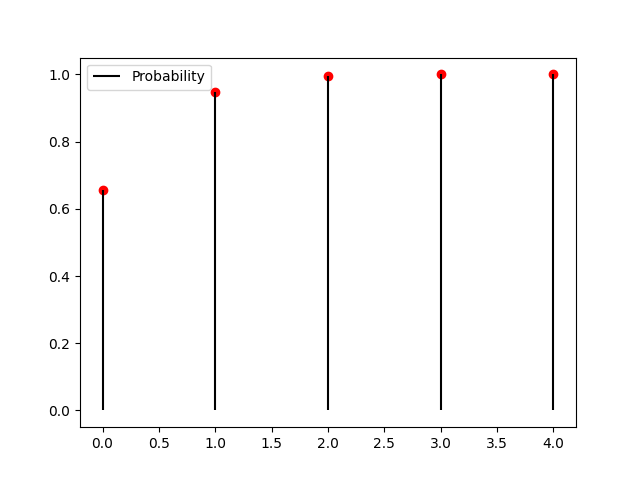
\includegraphics[width=\textwidth,height=5.5cm,keepaspectratio]{cdf.png}
		\caption{Cumulative Distribution Function}
		\label{fig}
	\end{figure}
\end{frame}
\begin{frame}
\begin{figure}[!ht]
		\centering
		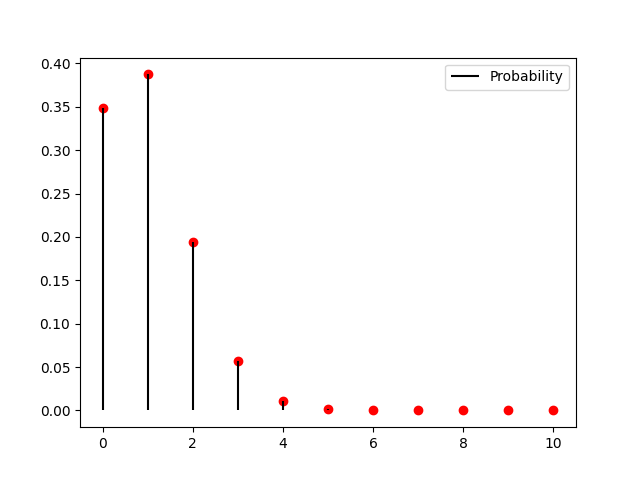
\includegraphics[width=\textwidth,height=5.5cm,keepaspectratio]{pmf.png}
		\caption{Probability Mass Function}
		\label{fig1}
	\end{figure}


\end{frame}
\end{document}